\section{Results}

\subsection{The verifier's labels lift both architectures}
\label{sec:main}
\begin{table}[t]
\centering\footnotesize\setlength{\tabcolsep}{4pt}
\caption{Localization and end-to-end accuracy (\%) on 188 verified cases, five folds with every trajectory in one fold. Training on the verifier's labels lifts both architectures on both metrics; the paired test separates neither trained variant from the other. $t$ is the step index at which the need arises; \emph{net} counts the cases the scorer gets right and the row's condition gets wrong, minus the reverse, with the two-sided McNemar $p$. Prompted full history and the screen index read in their own single call; both per-screen scorer rows and the trained full-history reader use read with history.}
\label{tab:main}
\resizebox{\linewidth}{!}{%
\begin{tabular}{llrrrrrr}
\toprule
 & & \multicolumn{3}{c}{localization} & \multicolumn{2}{c}{end-to-end} & scorer vs.\ row \\
\cmidrule(lr){3-5}\cmidrule(lr){6-7}
 & condition & all & $t\le15$ & $t\ge16$ & all & $t\ge16$ & loc: net, $p$ \\
 & & \multicolumn{3}{c}{$n$: 188 / 75 / 113} & 188 & 113 & \\
\midrule
\multirow{3}{*}{prompted} & full history & 54.8 & 68.0 & 46.0 & 31.4 & 20.4 & $+$33, $<$0.001 \\
 & screen index~\citep{readagent} & 41.0 & 48.0 & 36.3 & 23.9 & 25.7 & $+$59, $<$0.001 \\
 & per-screen scorer & 50.0 & 68.0 & 38.1 & 35.1 & 30.1 & $+$42, $<$0.001 \\
\midrule
\multirow{2}{*}{trained} & full history & 65.4 & 76.0 & 58.4 & 42.6 & 39.8 & $+$13, 0.086 \\
 & \textbf{per-screen scorer} & \textbf{72.3} & \textbf{80.0} & \textbf{67.3} & \textbf{44.7} & \textbf{42.5} & \\
\bottomrule
\end{tabular}}
\end{table}

Table~\ref{tab:main} separates the two things our method changes. Training the full-history reader on the verifier's labels lifts localization from 54.8\% to 65.4\% (net $+20$ cases, \pval{0.019}); training the per-screen scorer lifts it from 50.0\% to 72.3\% (net $+42$, $p<0.001$). Both gains come from labels that cost one substring test per screen. The supervision also reverses the ordering of the two architectures: prompted, the per-screen scorer trails full history by 4.8 points; trained, it leads by 6.9. A paired test on all 188 cases does not separate the two trained variants (net $+13$, \pval{0.086}), so we do not claim the decomposition alone wins. Figure~\ref{fig:results}(b) shows the two training effects side by side.

End-to-end accuracy tells the same story with a smaller spread. The trained full-history reader types the right text in 42.6\% of cases against 31.4\% for its prompted counterpart (net $+21$, \pval{0.003}), and the trained scorer reaches 44.7\% against 35.1\% for its own prompted counterpart under the same reader (net $+18$, \pval{0.001}). The paired test again does not separate the two trained variants (net $+4$, \pval{0.45}). Supervision is worth 9.6 and 11.2 points end-to-end to the two architectures, and the decomposition a further 2.1. At $t\ge20$ ($n=27$, not shown) the trained full-history reader leads on both metrics, 44.4\% and 33.3\% against the scorer's 37.0\% and 29.6\%.

Training helps the scorer twice as much as the full-history reader ($+22.3$ against $+10.6$), for which a likely reason is the label count: the per-screen format turns 188 cases into 2,861 labeled decisions.

\paragraph{Takeaway.} The verifier's labels carry the result. They lift a one-call reader by 10.6 localization points and a per-screen scorer by 22.3, and the two trained variants end within 2.1 points of each other end-to-end.

\subsection{The decomposition pays at gaps of 8--12 screens}
\label{sec:gap}
\begin{figure}[t]
\centering
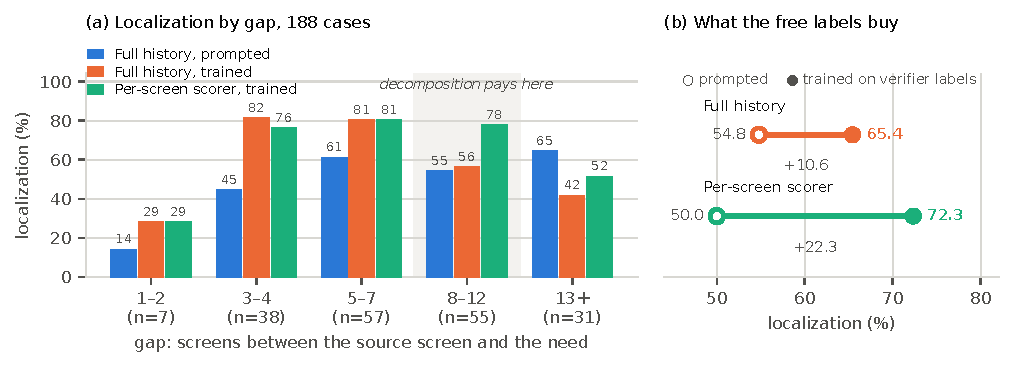
\includegraphics[width=\linewidth]{figures/fig2_results.pdf}
\caption{(a) Localization by gap. The trained variants are level everywhere except at gaps of 8--12 screens, where the per-screen scorer leads by 21.8 points; at 13 or more both fall below prompted full history. (b) What the free labels buy: the same labels lift both architectures, the scorer twice as much. Numbers are in Tables~\ref{tab:main} and~\ref{tab:gap}.}
\label{fig:results}
\end{figure}

\begin{table}[t]
\centering\footnotesize\setlength{\tabcolsep}{4pt}
\caption{Localization (\%) by gap, 188 cases. The trained variants are level except at gaps of 8--12 screens. At gaps of 13 or more both fall below prompted full history.}
\label{tab:gap}
\resizebox{\linewidth}{!}{%
\begin{tabular}{lrrrrr}
\toprule
gap (screens) & $n$ & full history, prompted & full history, trained & \textbf{per-screen scorer} & scorer vs.\ trained FH \\
\midrule
1--2 & 7 & 14.3 & 28.6 & 28.6 & $+$0, 0.48 \\
3--4 & 38 & 44.7 & \textbf{81.6} & 76.3 & $-$2, 0.72 \\
5--7 & 57 & 61.4 & 80.7 & \textbf{80.7} & $+$0, 0.77 \\
8--12 & 55 & 54.5 & 56.4 & \textbf{78.2} & $+$12, \textbf{0.003} \\
13$+$ & 31 & \textbf{64.5} & 41.9 & 51.6 & $+$3, 0.58 \\
\bottomrule
\end{tabular}}
\end{table}

Figure~\ref{fig:results}(a) and Table~\ref{tab:gap} show one band where the architectures diverge. Up to 7 screens back the trained full-history reader matches the scorer, and both improve on prompting by 14 points at gaps of 1--2 ($n=7$, too few to read anything into), 32--37 at 3--4 and 19 at 5--7. At gaps of 8--12 the trained full-history reader stops improving (56.4\%, within 2 points of prompted) while the scorer reaches 78.2\% (net $+12$, \pval{0.003}). This is the band where a single call must weigh a dozen candidates that the task description does not distinguish, and where scoring each screen on its own text pays.

Beyond 12 screens both trained variants fall below prompted full history (41.9\% and 51.6\% against 64.5\%, $n=31$). Training on 188 cases whose gaps have median 5 teaches a prior over distance that misfires at the tail, and the scorer inherits it; the no-distance ablation of Section~\ref{sec:ablation} does not fix the band either. We report this as the method's clearest failure.

\paragraph{Takeaway.} Per-screen scoring is not uniformly better than one call over the history. It wins where the candidate set is large and undifferentiated, and both trained variants lose to prompting at the longest gaps.

\subsection{An external sample confirms the margin over prompting}
\label{sec:ext}
\begin{table}[t]
\centering\footnotesize\setlength{\tabcolsep}{4pt}
\caption{External set: 93 cases from a fourth sample of 400 trajectories, mined after we fixed every design decision. We train each condition on all 188 cross-validated cases and evaluate once. $p$ is against the trained per-screen scorer.}
\label{tab:ext}
\resizebox{\linewidth}{!}{%
\begin{tabular}{lrrrr}
\toprule
condition & localization & $p$ & end-to-end (read with history) & $p$ \\
\midrule
full history, prompted & 59.1 & 0.003 & 23.7 & $<$0.001 \\
screen index, prompted & 37.6 & $<$0.001 & -- & \\
per-screen scorer, prompted & 41.9 & $<$0.001 & -- & \\
full history, trained & 76.3 & 0.63 & 51.6 & 0.62 \\
\textbf{per-screen scorer, trained} & \textbf{79.6} & & \textbf{49.5} & \\
\quad scorer with single-screen read & & & 37.6 & 0.016 \\
\bottomrule
\end{tabular}}
\end{table}

Table~\ref{tab:ext} repeats the comparison on cases that no design decision saw. The scorer localizes 79.6\% against 59.1\% for prompted full history (net $+19$, \pval{0.003}) and 37.6\% for the prompted index (net $+39$, $p<0.001$); the untrained scorer reaches 41.9\%. The trained full-history reader reaches 76.3\%, and the paired test again does not separate it from the scorer (\pval{0.63}), reproducing Section~\ref{sec:main} out of sample. End-to-end, read with history raises accuracy from 23.7\% for prompted full history to 51.6\% for the trained full-history reader (net $+26$, $p<0.001$) and 49.5\% for the scorer, which again the paired test does not separate (net $-2$, \pval{0.62}); the scorer with a single-screen read reaches 37.6\%.

The external needs sit at steps 12--15 (72 cases), 16--19 (19) and 20 or later (2), so this sample tests the mid-range. At 12--15 the scorer localizes 61 of 72 against prompted full history's 42; at 16--19 the two are within one case (12 and 13 of 19).

\paragraph{Takeaway.} On data held out from every design decision, verifier supervision keeps a 20-point margin over prompting, and the two trained variants remain indistinguishable.

\subsection{Ablations and read-stage controls}
\label{sec:ablation}
\begin{table}[t]
\centering\footnotesize\setlength{\tabcolsep}{4pt}
\caption{Left: scorer ablations, localization (\%) on 188 cases, $p$ against the full scorer. Right: read-stage controls, end-to-end (\%) on the same cases, $p$ against marking the scorer's choice.}
\label{tab:abl}
\resizebox{\linewidth}{!}{%
\begin{tabular}{lrr@{\hspace{2em}}lrr}
\toprule
scorer ablation & loc & $p$ & read stage (marked screen) & e2e & $p$ \\
\midrule
full scorer (7B, distance, weight 3) & \textbf{72.3} & & gold source screen marked & \textbf{45.2} & 1.00 \\
no distance in the prompt & 70.7 & 0.61 & \textbf{scorer's choice} & \textbf{44.7} & \\
positive weight 1 & 72.3 & 0.77 & scorer's top two & 45.2 & 1.00 \\
3B base model & 68.1 & 0.22 & most recent screen & 38.8 & 0.10 \\
\quad 3B at $t\ge20$ & \textbf{48.1} & & random earlier screen & 36.7 & 0.018 \\
\bottomrule
\end{tabular}}
\end{table}

Table~\ref{tab:abl} shows the design is insensitive to its prompt and loss settings. Removing the distance from the prompt costs 1.6 points (\pval{0.61}) without rescuing the 13$+$ band, and the positive weight leaves localization at 72.3\%. A 3B base loses 4.2 points overall while gaining 11.1 at $t\ge20$ (48.1\% against 37.0\%).

The read-stage controls bound what marking buys. Marking the gold source screen gives 45.2\% against the scorer's 44.7\%, so the scorer sits at this reader's ceiling, and marking its top two adds nothing. Marking the most recent screen gives 38.8\% and a random earlier screen 36.7\% (\pval{0.018}): repeating any screen accounts for 5--7 of the 13 points over prompted full history, and the chosen screen for the rest.

\subsection{Where the index route stops, and two mandatory filters}
\label{sec:index}
\begin{table}[t]
\centering\footnotesize\setlength{\tabcolsep}{4pt}
\caption{Short set ($n=85$), localization (\%). The screen index's writer cannot pass full history, and an oracle that rewrites only the source screen's line reaches full-history level and no higher.}
\label{tab:index}
\resizebox{\linewidth}{!}{%
\begin{tabular}{lr@{\hspace{2em}}lr}
\toprule
condition & loc & writer variant / oracle & loc \\
\midrule
no history (end-to-end 2.4) & n/a & writer trained with DPO on the same 85 cases & 45.9 \\
full history, prompted & 65.9 & writer forced to a two-field format & 47.1 \\
per-screen summary & 23.5 & writer allowed to copy values & 49.4 \\
screen index, prompt-only & 49.4 & writer: three lines per screen & 43.5 \\
BM25, task $+$ current screen as query & 10.6 & writer: retrieval prompt, sampled, every screen & 44.7 \\
BM25, gold text as query & 92.9 & oracle: source line replaced by 1 of 5 sampled lines & 58.8--65.9 \\
\textbf{per-screen scorer, trained} & \textbf{77.6} & oracle: best of the five sampled lines per case & 76.5 \\
\bottomrule
\end{tabular}}
\end{table}

We built the screen index first; Table~\ref{tab:index} records why we left it. The prompt-only index localizes 49.4\% against 65.9\% for full history (\pval{0.035}). We trained its writer with direct preference optimization~\citep{dpo} on 224 preference pairs built from the same 85 cases that we score it on, a choice that favors it. It localizes 45.9\%, and four prompt variants stay between 43.5\% and 49.4\%. An oracle that replaces only the source screen's line with one of five lines sampled at temperature 0.9 gives 58.8--65.9\%, level with full history ($p\ge0.36$). The best of the five per case gives 76.5\%, but 64\% of cases are insensitive to which line it uses, so that gain is redundancy no single writer realizes. BM25 localizes 92.9\% with the gold text as query and 10.6\% with what the agent actually knows: the difficulty is deciding what to look for, which a 32-token line does not ease.

\paragraph{Two filters move conclusions more than any method.} \emph{Earliest-source scoring} labels only the earliest screen that contains the text, but 47\% of short-set cases have two or more; scoring any valid screen lifts the index 15.3 points and full history 11.8. \emph{Current-screen leakage} admits cases whose answer is also on the current screen (28\% of short-set and 58\% of long-set candidates). On the 127 unfiltered long-set cases a rule that reads only the two previous screens beats full history by 17.3 points (\pval{0.010}); on the 53 clean ones it loses by 22.7 (\pval{0.019}). We found this by noticing that the rule's localization gain did not move end-to-end accuracy, and we retracted the result. Both filters are one condition each: at mining time the answer must be absent from the current screen's OCR, and at scoring time any screen whose OCR contains the answer counts as correct.

\subsection{Limits}
\label{sec:limits}
Gaps of 13 or more screens are the method's clearest failure: both trained variants fall below prompted full history and no ablation recovers the band. At $t\ge20$ ($n=27$) the 7B scorer matches prompted full history (37.0\%), while the trained full-history reader reaches 44.4\% and a 3B scorer 48.1\%, so neither our preferred variant nor its size is the right choice at the longest histories. We cross-validate on one dataset with one OCR engine, and the external set comes from the same corpus. The training labels and the localization metric are the same substring check, so training points the scorer at the metric we score it on; a spot check of 20 verified cases found that every labeled screen did show the needed text, and that in 5 of them the agent had typed the text itself earlier (a search query or a note title), which makes the need weaker in those 5. Each condition is a single training run, so our paired tests account for case-level variance only. The scorer's maximum probability predicts whether its localization is correct with an area under the ROC curve of 0.768; falling back to prompted full history below 0.5 raises localization to 75.0\%, which we report but do not use.
